\chapter{Domain Analysis}
\label{cha:analysis}

This chapter analyses the concepts of service and service decomposition in more detail and concludes with a market overview on different service decomposition approaches. 

\section{What is a Service?}
\label{sec:serviceIntro}

\textit{Service} is one of the most used terms in the field of software architecture and has been defined differently in many papers, books, and blog posts in numerous ways and various contexts. This section consolidates multiple definitions and defines what a Service in context of this thesis is.

\subsection{Different Views on Services}

The \enquote{4+1 View Model of Software Architecture} by Philippe Kruchten\cite{fourPlusOne} describes software architecture using multiple views such as the \textit{Logical}, \textit{Physical}, \textit{Development}, and \textit{Process View}, illustrated by \textit{Scenarios}. During the research for this thesis we discovered that the difficulty to clearly define the word service lies in the fact that different definitions focus on contrasting views. For this thesis we use multiple definitions for the word service depending if we talk about the \textit{logical} or the \textit{physical} view of a service.

\subsubsection{Logical Service}

\begin{quotation}
A service is the technical authority for a specific business capability --- Udi Dahan\cite{serviceDefinitionDahan}
\end{quotation}
   
This definition focuses more on the logical or scenario view of a service than its technical representation. All data and rules required to fulfill a business specification are owned by one and only one service. 

Udi Dahan implies that a service is not restricted to a specific application, process, technology or layer. In fact it contains required layers itself, including databases, logic, and \gls{UI} code.

A logical service is autonomous and composed from many processes, webservices or databases, but keeps a clear boundary and interface against the outer world. Communication with other parts of the system only happens on a well defined interface on a common communication channel.

\subsubsection{Bounded Context}

Another concept describing logical services is the bounded context as defined in the Domain-Driven Design:\cite{evans2014domain}

\begin{quotation}
	A description of a boundary (typically a subsystem, or the work of a particular team) within which a particular model is defined and applicable.
\end{quotation}

A model only used within one bounded context is defined and visible only in that context. Accordingly a model used in multiple services needs to have a globally shared definition, defined as \textit{Published Language} in the context of \gls{DDD}\cite{evans2014domain}:

\begin{quotation}
	The translation between the models of two bounded contexts requires a common Language.
\end{quotation}

The process of service decomposition as done by the Service Cutter automatically defines the published language of the system. 

\subsubsection{Physical Service}

Martin Fowler describes a service as following:

\begin{quotation}
	A service will be used remotely through some remote interface, either synchronous or asynchronous.\cite{fowlerIoC}
\end{quotation}

This definition by Martin Fowler is based on the physical structure and is close to what recently has been advertised as a \textit{Microservice}:

\begin{quotation}
	In short, the microservice architectural style is an approach to developing a single application as a suite of small services, each running in its own process and communicating with lightweight mechanisms, often an HTTP resource API.\cite{fowlerMicroservice}
\end{quotation}


A process providing a remote API might provide business logic, pure technical functionality or a data store. A service commonly includes at least a data store, wrapped by a RESTful HTTP API. Physical services might be congruent with logical services but very often more complex cases split logical services in multiple physical services. 

\subsubsection{Should a Service Cutter produce Logical or Physical Service Candidates?}

While every logical reason to define service boundaries applies to logical and physical services, technical reasons like technology constraints might define additional physical service boundaries. Infrastructure or deployment constraints might lead to multiple logical services deployed into one physical service. %TODO discuss: "Infrastructure or deployment constraints" such as?

We do not strictly define what kind of services the Service Cutter suggests. Given that the Service Cutter mostly focuses on logical criteria it could well be that a suggested service needs to be further decomposed due to technological reasons.

%TODO ZIO: 2-3 examples for logical / phyiscal services (generally give examples for conecpts)
% Note Lukas: Logical service containing three layers (DB, logic, GUI)each on a single process

\subsection{Nanoentities, Building Blocks for Services}


A service incorporates two elements:

\begin{description}
	\item[Data] A service has ownership over some of the system's data. It is the only instance responsible for changes on that data and optionally informs other services about changes. The data is often, but not necessarily, stored in a database. Data which is published to other services belongs to the published language of the system.
	\item[Operations] A service has ownership over business rules and calculation logic. These operations are often based on the data the service owns.
\end{description}

Within the Service Cutter, both elements are unified under the term \textit{nanoentity}. A nanoentity is a piece of information, either in form of a data field or an operation result. Examples for possible nanoentities are illustrated in Figure \ref{fig:nanoentities}.

Each service must embody both, data and operations, to be considered as a service. Something only providing CRUD\footnote{Create, Read, Update, and Delete} functions on data is considered a database. Something only providing operations is considered a function, not a service. 

Service decomposition therefore is the act of defining a number of services and assigning all nanoentities to the responsible service. 

The factors driving the decomposition are discussed in more detail in the next section.


\begin{figure}[H]
	\centering{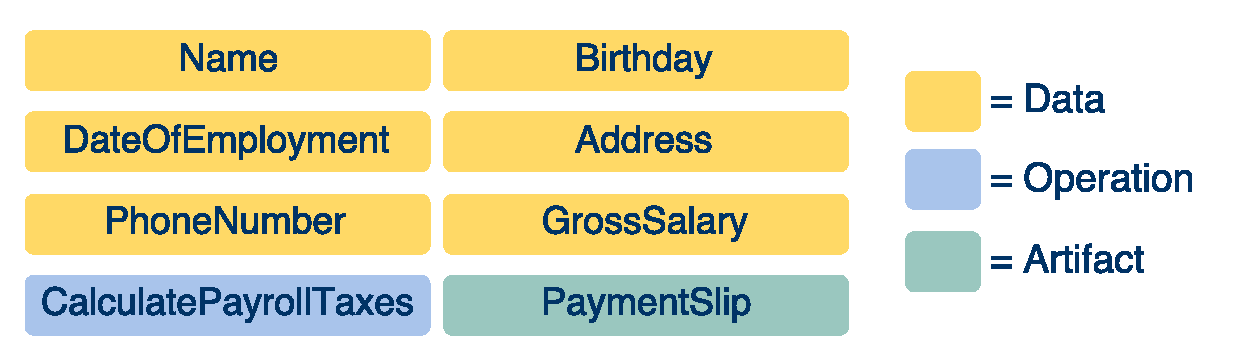
\includegraphics[scale=0.5]{diagrams/Nanoentities.pdf}}
	\caption{Nanoentities related to an employee}
	\label{fig:nanoentities}
\end{figure}

\section{Driving Factors for Service Decomposition}

Well experienced software architects decompose systems by reason of multiple factors to ensure a maintainable, robust and consistent system with business relevance and good performance. This section describes the factors mostly considered by architects. 

Decomposition has been a main discipline for programmers since early in the history of our industry. David L. Parnas published a paper entitled \enquote{On the Criteria To Be Used in Decomposing Systems into Modules} in 1972\cite{parnaDecomposing}. Shortly after, the terms \textit{coupling} and \textit{cohesion} as software design metrics appeared as part of the \textit{Structured Design} technique\cite{structuredDesign}:

\begin{description}
	\item[Coupling] A measure of how closely connected two routines or modules are.\newline In	software design, a measure of the interdependence among modules in a computer program.\cite{softwareVocabulary}
	\item[Cohesion] The manner and degree to which the tasks performed by a single software module are related to one another. \newline 
	In software design, a measure of the strength of association of the elements within a module.\cite{softwareVocabulary}
\end{description}

Software architects commonly started to use this metrics to define good architectures as having high cohesion within and low coupling between its parts. R. C. Martin later described a general principle to achieve loose coupling and high cohesion:

\begin{description}
	\item[Single Responsibility Principle] Gather together the things that change for the same reasons. Separate those things that change for different reasons.\cite{SRP}
\end{description}

Starting from these principles, we analyzed different types and reasons for coupling and cohesion metrics and created the decomposition model described in the next Chapter.


\section{Existing Decomposition Solutions}

TODO: Market analysis. Java Code analysis, GraphGist project to analyse service dependencies etc... %TODO

SOMA, one more SOA method

OOAD, 

DDD

output of these methods is SC input! (model)


